\documentclass{article}
\usepackage{ctex}
\usepackage[english]{babel}
\usepackage[margin=1in]{geometry}
\usepackage{amsmath,graphicx,xcolor,alltt,theorem}
\usepackage{lmodern}

\begin{document}

\title{SPIV Configuration in Pinhole Camera Model}
\author{ Liu Ning }
\maketitle

\section{SPIV translation configuration}

\subsection{双相机布置}

\begin{figure}[htbp]
  \centering
  \raisebox{0.0\height}{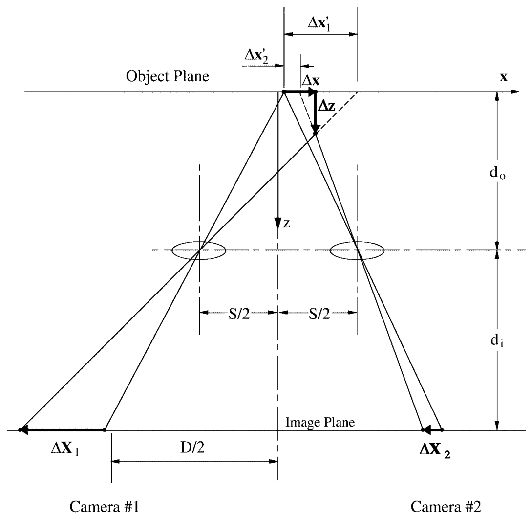
\includegraphics[width=9cm,height=8cm]{./figures/optical_route-1.pdf}}
  \caption{Schematic of stereocamera in the translation configuration.}
\end{figure}

\subsection{双二维像重构实际三维空间}

附录中提供了双相机object plane中二维像重构世界坐标系空间的映射关系,$\Delta \mathbf{X}_{left~  camera}$ 和$\Delta \mathbf{X}_{right~camera}$在上述代码中对应\textbf{dXl}和\textbf{dXr},分别表示实际三维距离矢量在object plane (对应激光面)中的投影
\footnote{注意此处没有讨论成像平面上的投影。在平行布置的情况下,object、lens和image三者平面平行,object plane 上的距离投影矢量$\Delta \mathbf{x_o}$与image plane上的距离投影矢量$\Delta \mathbf{x_i}$满足$\Delta \mathbf{x_o} / d_o = - \Delta \mathbf{x_i} / d_i$(相似三角形)。 后续通过像平面(照片上反映)的距离反算真实三维空间的距离并无难度,因此推导到此为止。}。
两个矢量的第一项可与$\Delta X_{ {left}}$和$\Delta X_{ {right}}$构成两个线性方程组,

\begin{align}
   - \frac{d_o  \left( \frac{S}{2} + x \right)}{d_o - z} + \frac{d_o  \left(
   \Delta x_{ {world}} + \frac{S}{2} + x \right)}{- \Delta
   z_{ {world}} + d_o - z} & = \Delta X_{ {left}},\\
   - \frac{d_o  \left( - \frac{S}{2} + x \right)}{d_o - z} + \frac{d_o 
   \left( \Delta x_{ {world}} - \frac{S}{2} + x \right)}{- \Delta
   z_{ {world}} + d_o - z} & = \Delta X_{ {right}} .
\end{align}
求解得到世界坐标系下的$\Delta x_{ {world}}$和$\Delta z_{ {world}}$为
\begin{align}
     \Delta x_{ {world}} = & \frac{\Delta X_{ {left}} (x - S / 2) -
     \Delta X_{ {right}} (x + S / 2)}{- S - (\Delta X_{ {left}} -
     \Delta X_{ {right}})},\\
     \Delta z_{ {world}} = & \frac{- d_o (\Delta X_{ {left}} - \Delta
     X_{ {right}})}{- S - (\Delta X_{ {left}} - \Delta
     X_{ {right}})} .
\end{align}
而两个矢量的第二项可以分别独立求解世界坐标系下的$\Delta y_{ {world}}$,
\begin{align}
     - \frac{d_o y}{d_o - z} + \frac{d_o  (\Delta y_{ {world}} + y)}{-
     \Delta z_{ {world}} + d_o - z}  & = \Delta Y_{ {left}},\\
     - \frac{d_o y}{d_o - z} + \frac{d_o  (\Delta y_{ {world}} + y)}{-
     \Delta z_{ {world}} + d_o - z} & = \Delta Y_{ {right}} .
 \end{align}
将二者的求解结果取平均以提高结果的精确性,
\begin{align}
\Delta y_{ {world}} = \frac{- y \Delta z_{ {world}}}{d_o} + \frac{1}{2} \cdot (\Delta Y_{ {left}} + \Delta Y_{ {right}}) \left( 1 - \frac{\Delta z}{d_o} \right) .
\end{align}
至此,颗粒的实际距离矢量$\left[\begin{array}{c} \Delta x_{ {world}} \quad \Delta y_{ {world}} \quad \Delta z_{ {world}} \end{array}\right]^T$均已求出。

如何确定世界坐标系下的$x, y$?

\section{SPIV angular-displacement configuration}

\begin{figure}[htbp]
  \centering
  \raisebox{0.0\height}{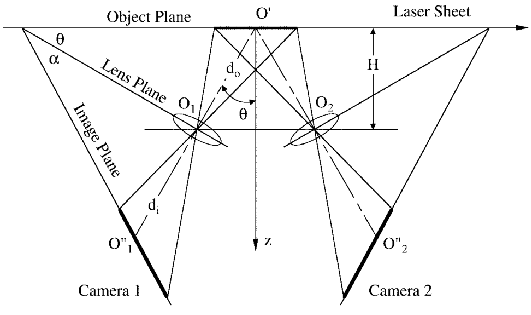
\includegraphics[width=9cm,height=5cm]{./figures/optical_route-2.pdf}}
  \caption{Schematic of stereocamera in the angular-displacement
  configuration.}
\end{figure}

\begin{figure}[htbp]
  \centering
  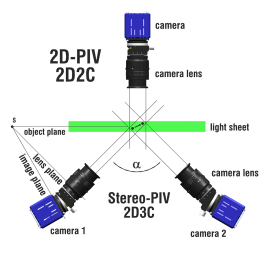
\includegraphics[width=.4\textwidth]{./figures/lavision-Stereo-PIV.png}
  \caption{Lavision Stereo-PIV system.}
\end{figure}

\subsection{沙姆定律( Scheimpflug principle)}

\begin{figure}[htbp]
  \centering
  \raisebox{0.0\height}{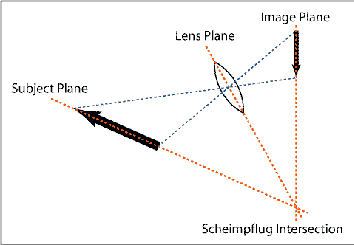
\includegraphics[width=6cm,height=4cm]{./figures/optical_route-3.pdf}}
  \caption{The angles of the Scheimpflug principle, using the example of a
  photographic lens.}
\end{figure}

\begin{figure}[htbp]
  \centering
  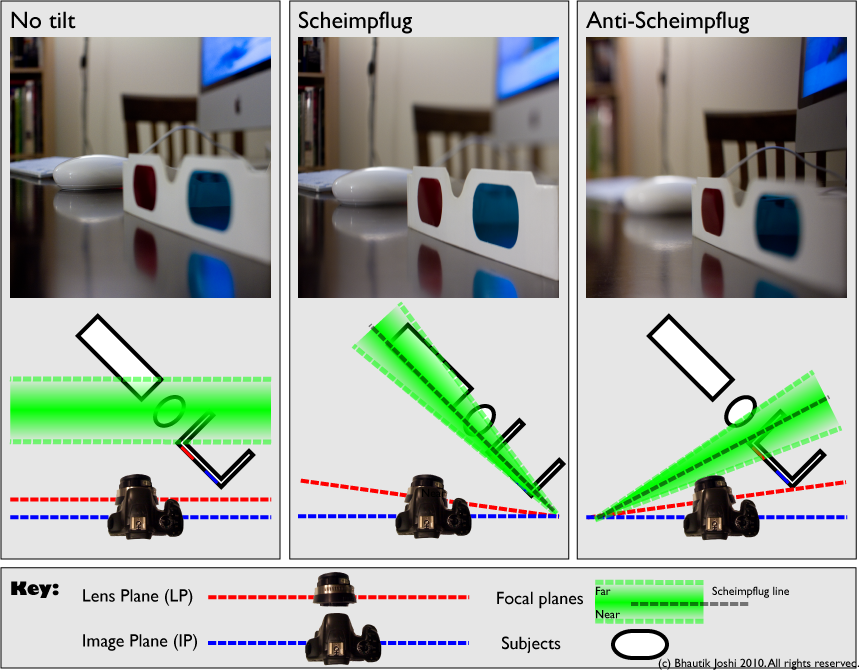
\includegraphics[width=0.6\textwidth]{./figures/tilt_camera.png}
  \caption{Illustration of the Scheimpflug principle.}
\end{figure}

只要满足成像、镜头、测量三个平面交于同一条直线(对于未移轴的镜头,认为三个平行平面相 交于无限远处)的条件,则可以保证测量平面的物体能够清晰成像,因此能够起到调整景深区域 位置的作用。

目的:
\begin{itemize}
  \item 增大公共景深区域(common focus area)
\end{itemize}

\begin{figure}[htbp]
  \centering
  \raisebox{0.0\height}{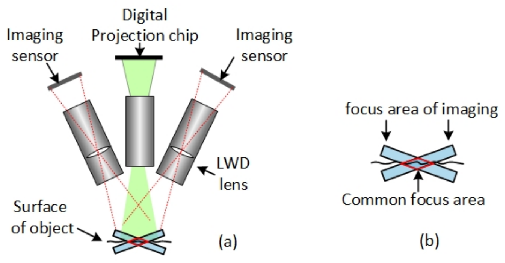
\includegraphics[width=10cm]{./figures/optical_route-4.pdf}}
  \caption{(a) The schematic of setup. (b) The common focus area (Marked with
  red quadrangle).}
\end{figure}

\begin{figure}[htbp]
  \centering
  \raisebox{0.0\height}{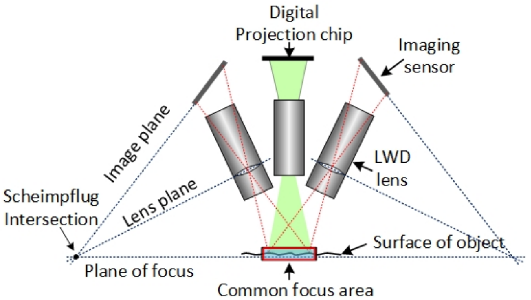
\includegraphics[width=10cm]{./figures/optical_route-5.pdf}}
  \caption{System design based on the Scheimpflug principle.}
\end{figure}

副作用:
\begin{itemize}
  \item 不均匀放大倍率 $\Longleftarrow \, \alpha \neq 0$
  
  \item 同侧布置两台相机畸变拉伸方向相反(oppositely
  stretched)
\end{itemize}

\subsection{$\alpha = 0$ condition: Image Plane // Lens Plane}

为满足$\alpha = 0$情况的成像条件,需要牺牲光圈\footnote{$f^{\#}$值越大,光圈越小,得到的景深$\delta z$越大。},增大景深,使其能够覆盖尽可能大的三维空间, 
\begin{align}
\delta z = 4 (1 + M_n^{- 1})^2 f^{\#^2} \lambda .
\end{align}
其中,$\lambda$为激光波长,$M_n = d_i / d_o$为相机放大倍率(Camera magnification)。

同侧对称布置下双相机的映射关系计算见附录。首先计算世界坐标系下距离矢量

上述方程组完整,一台相机的object plane数据可以直接求解三维矢量。但是相机照片并没有object plane中的所有分量信息,因此必须考虑如何从投影到image plane后的矢量信息重建三维空间。

在object plane中$\left[ X \quad Y \quad Z \right]_{\{ {left}, {right} \}}^T$映射到image plane为$\left[ x_i \quad y_i \quad z_i
\right]^T_{\{  {left},  {right} \}}$, 两者均在相机坐标系内,满足关系:
   $$
   \begin{aligned}
    x_i & =  - \frac{d_i}{Z} \cdot X\\
     y_i & =  - \frac{d_i}{Z} \cdot Y\\
     z_i & =  - d_{i}.
   \end{aligned}
   $$

\subsection{双相机异侧布置}

\begin{figure}[htbp]
  \centering
  \raisebox{0.0\height}{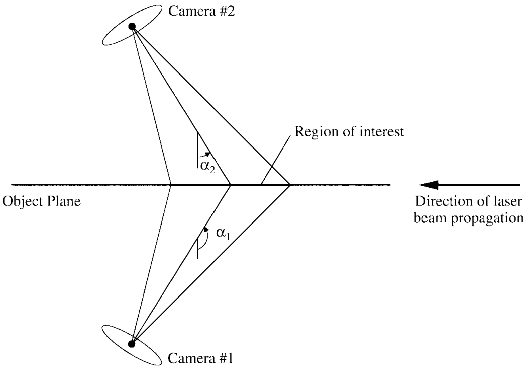
\includegraphics[width=9cm,height=6cm]{./figures/optical_route-6.pdf}}
  \caption{Stereoscopic arrangement with cameras on either side of the light
  sheet (adapted from Willert 1997).}
\end{figure}

优势:
\begin{itemize}
  \item 增大forward scatter,提高信噪比?
  
  \item 两台相机的畸变拉伸方向一致
\end{itemize}

\subsection{水棱镜}



\end{document}
